\setlength{\columnsep}{3pt}
\begin{flushleft}

	Below diagram shows important files and their short description relating to user \& group details:
	\begin{figure}[h!]
	\centering
	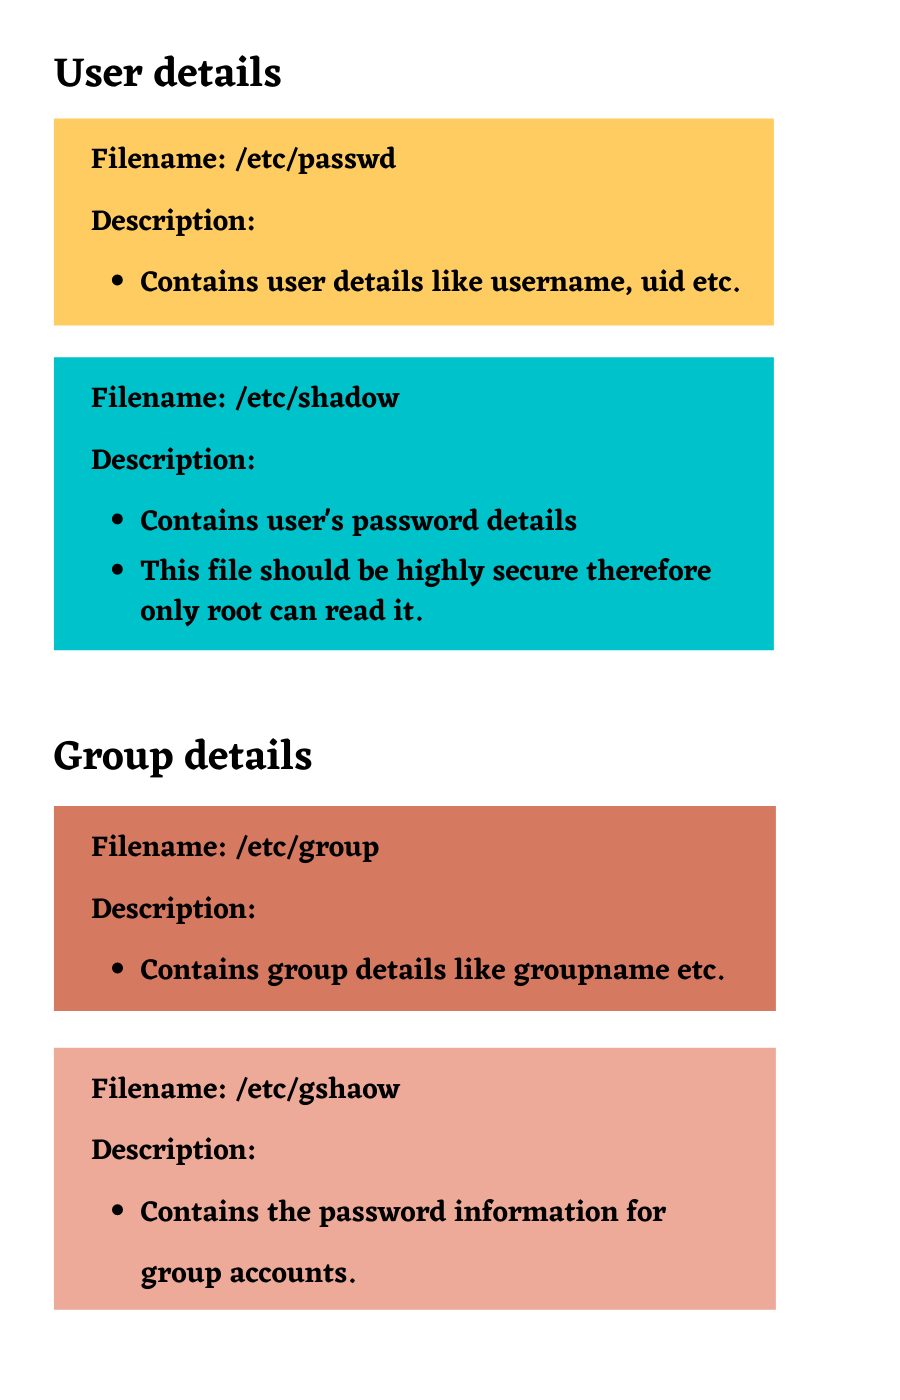
\includegraphics[scale=0.4]{content/chapter4/images/users6.png}
	\caption{Important user \& group files}
	\label{fig:prime_secondary_group12}
\end{figure}

Let's see each of these file in detail.

\newpage

\textbf{Structure of /etc/passwd file}
\begin{itemize}
	\item Fields in this file are separated by a ":" (colon).
	\begin{figure}[h!]
	\centering
	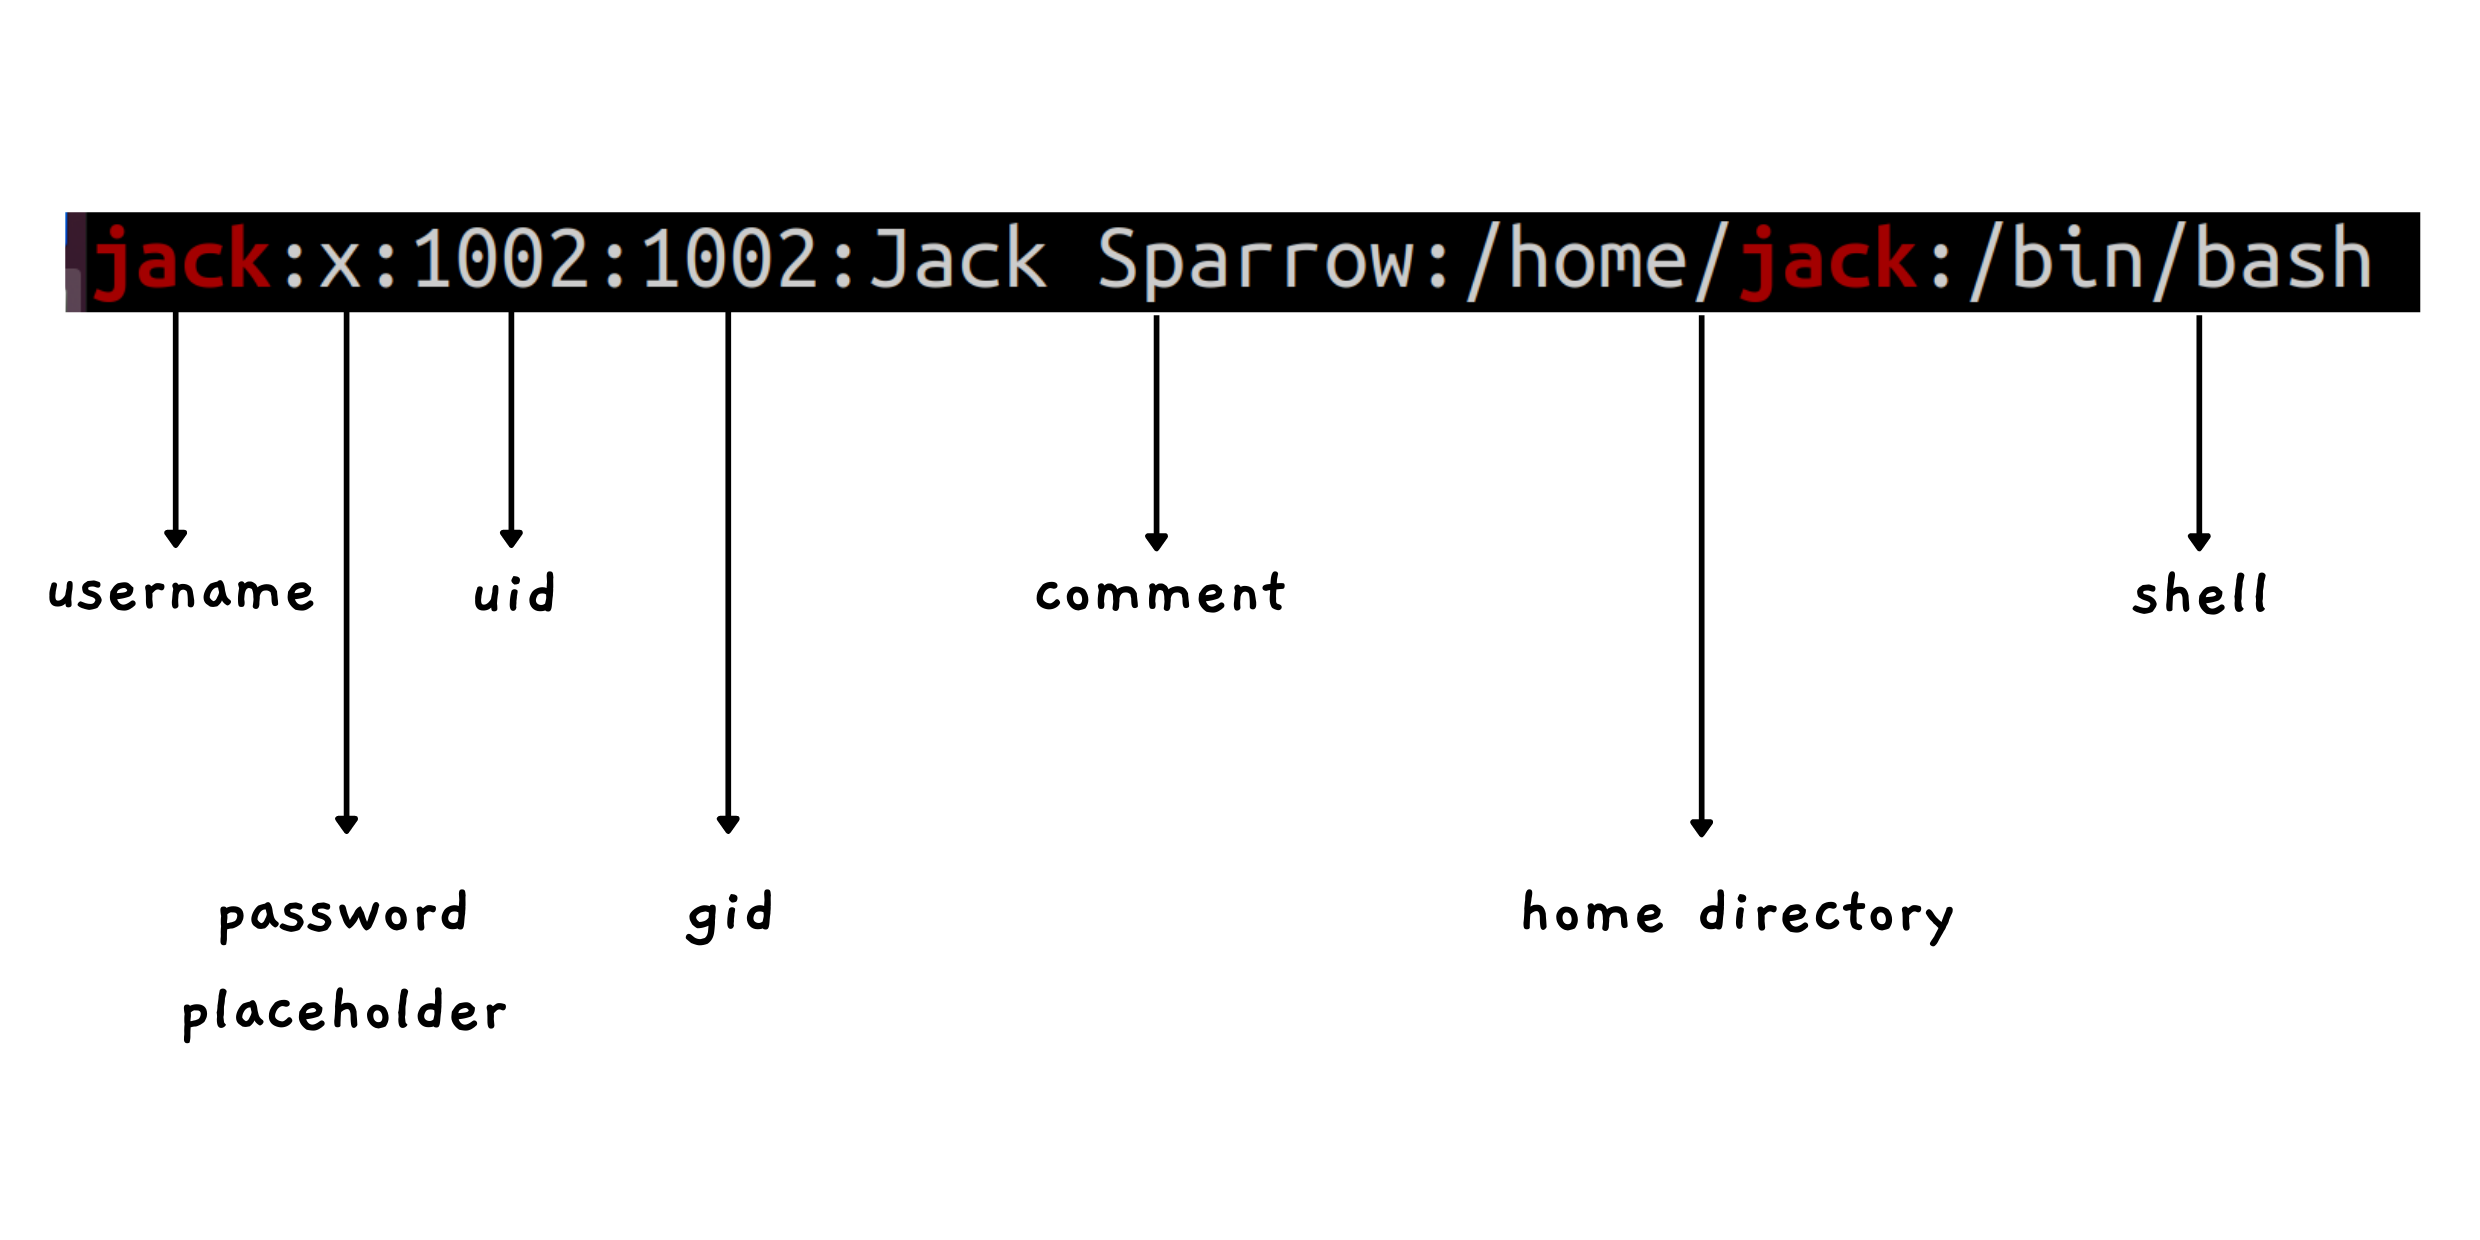
\includegraphics[scale=.2]{content/chapter4/images/53.png}
	\caption{Sample /etc/passwd entry}
	\label{fig:user_group1}
	\end{figure}	
	\newline
Explaination:
\begin{itemize}
		
	\item Column 1: \textbf{Username} - Name of the user. It is case-sensitive.
	\item Column 2: \textbf{Password placeholder} - "x" acts as placeholder. Encrypted password are now stored in \textbf{/etc/shadow} file.
	\item Column 3: \textbf{User ID}
	\item Column 4: \textbf{Group ID}
	\item Column 5: \textbf{Comment} - More description about user.
	\item Column 6: \textbf{Home directory} - Location of user's personal data.
	\item Column 7: \textbf{Shell} - User login shell, default is \textbf{/bin/bash}.
\end{itemize}


\end{itemize}	

\newpage

\textbf{Structure of the /etc/shadow file}
\begin{itemize}
	\item Fields in this file are separated by a ":" (colon).
	\begin{figure}[h!]
		\centering
		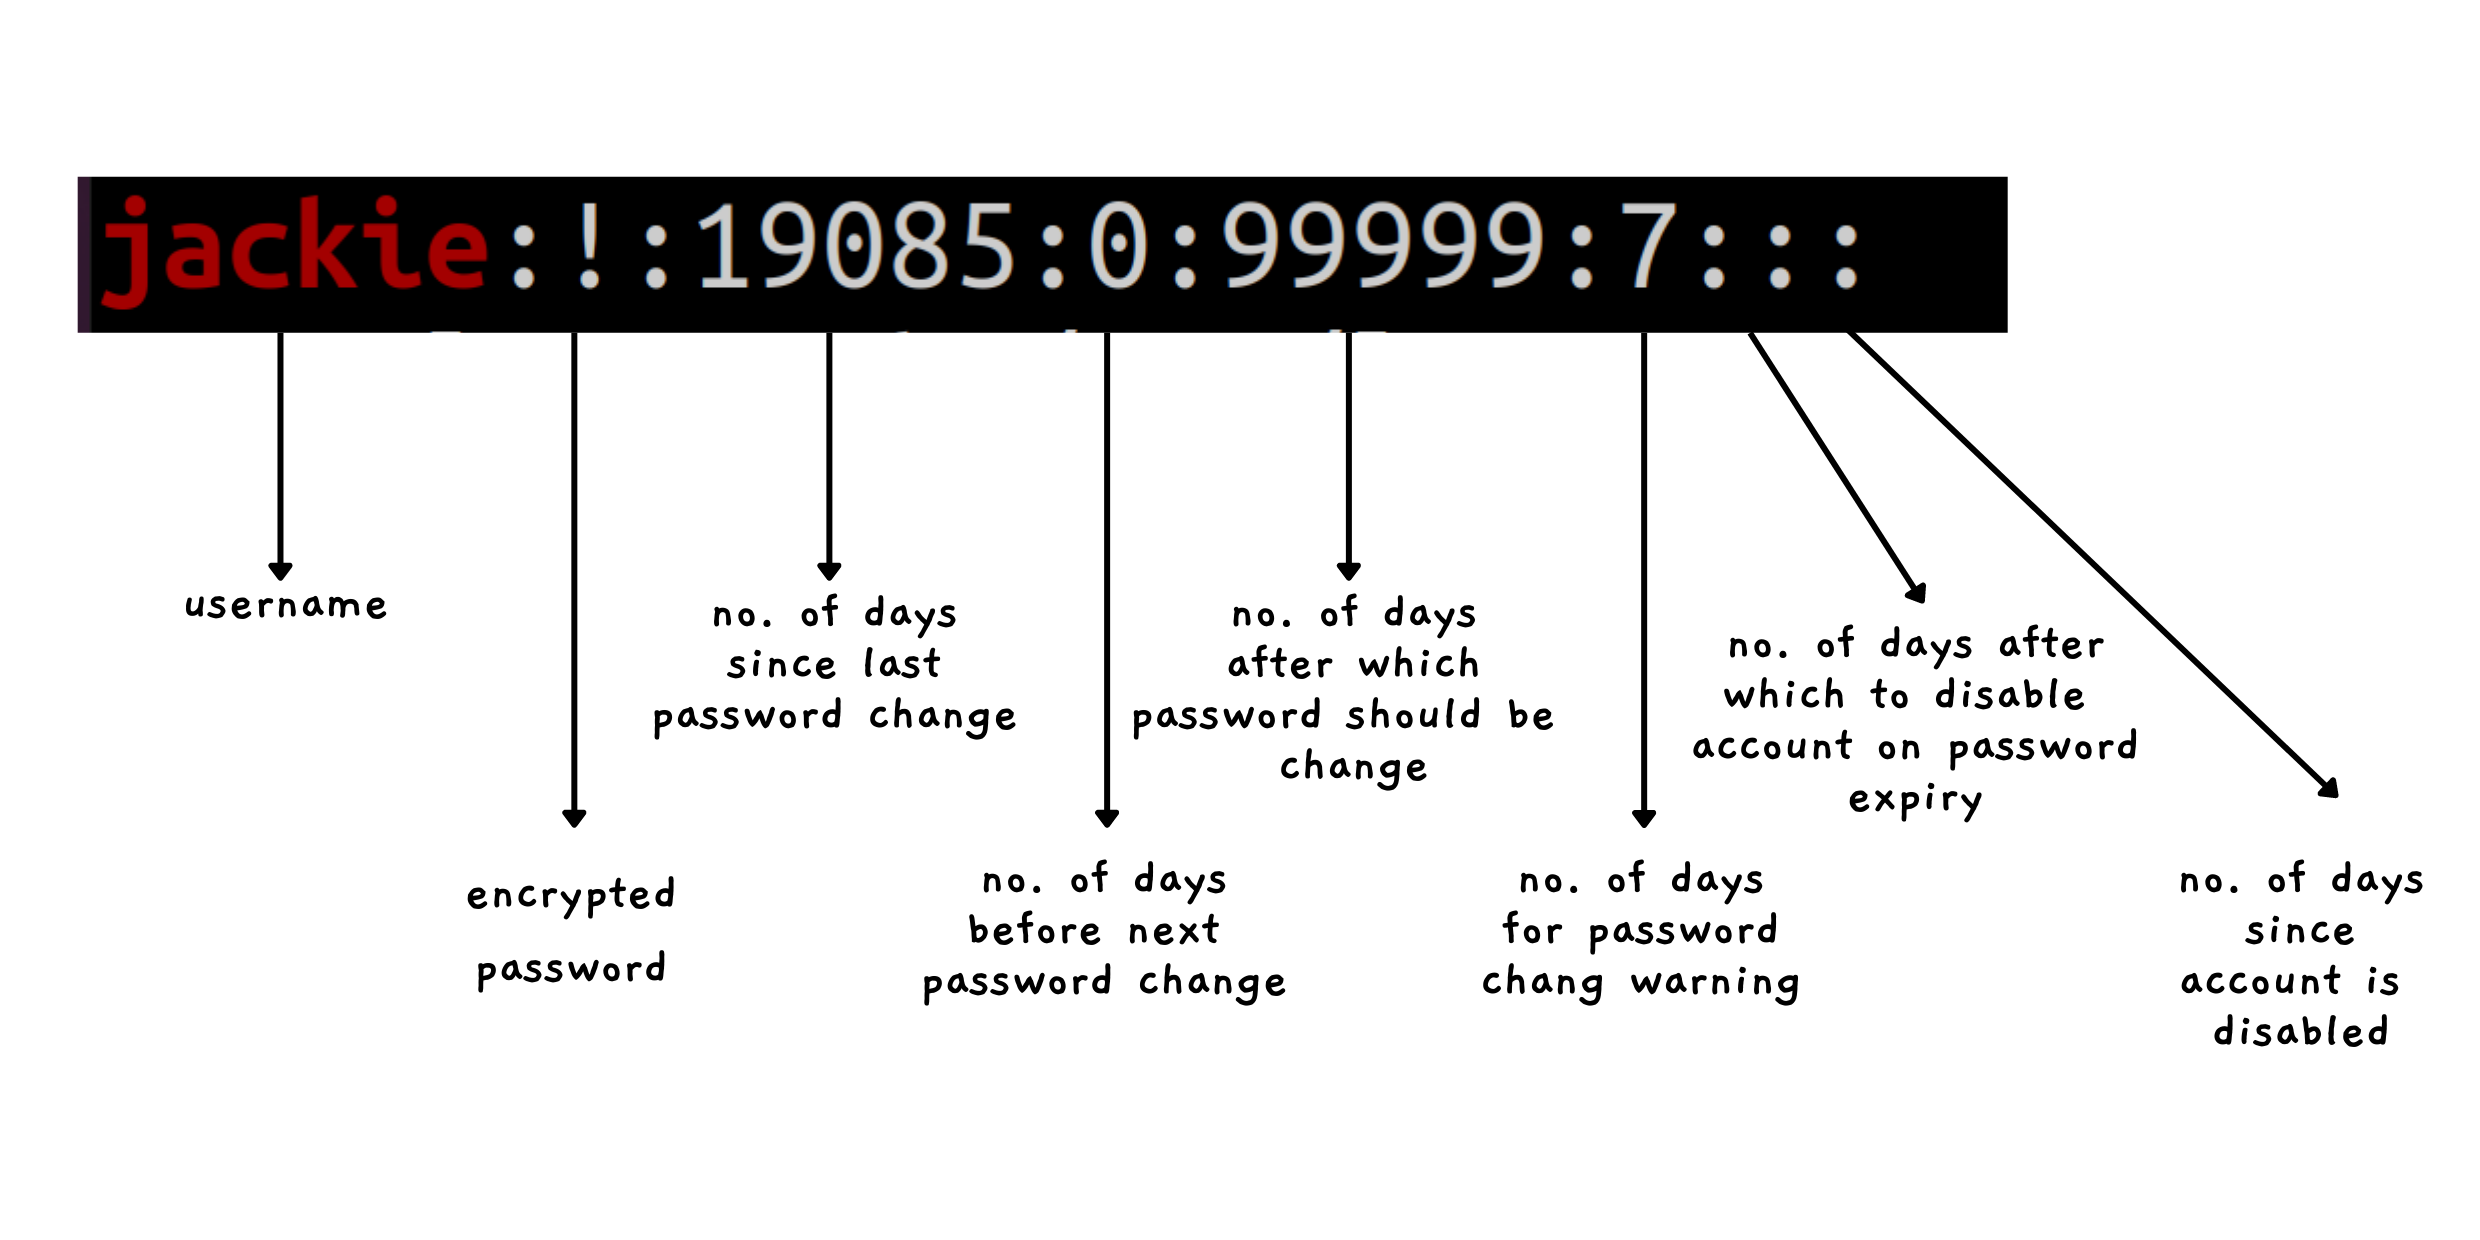
\includegraphics[scale=.2]{content/chapter4/images/55.png}
		\caption{Sample /etc/shadow entry}
		\label{fig:user_group}
	\end{figure}	
	\newline
	Explaination:
	\begin{itemize}
		\item Column 1: \textbf{Username} - A direct match to the username in the \textbf{/etc/passwd} file.
		\item Column 2: \textbf{Encrypted Password} - Store password in encrypted format.
		\bigskip
		\begin{tcolorbox}[breakable,notitle,boxrule=-0pt,colback=yellow,colframe=yellow]
			\color{black}
			\textbf{Note:} 
			\begin{itemize}
				\item \textbf{“!”} in this entry means the account is disabled or locked. 
				\item \textbf{“!!”} mask means password is not assigned.
			\end{itemize}
		\end{tcolorbox}
		
		
		
		\item Column 3: \textbf{Last password change} - The number of days (since January 1, 1970) since the password was last changed.
		\item Column 4: \textbf{Probable next password change} - The number of days before password may be changed (0 indicates it may be changed at any time).
		\item Column 5: \textbf{Next password change} - The number of days after which password must be changed (99999 indicates user can keep his or her password unchanged for many, many years).
		\item Column 6: \textbf{Password change warning} - The number of days to warn user of an expiring password (7 for a full week).
		\item Column 7:\textbf{Password expiry} - The number of days after password expires that account is disabled.
		\item Column 8: \textbf{Account disable} - The number of days since January 1, 1970 that an account has been disabled.
	\end{itemize}	
\end{itemize}	
	
\newpage

\textbf{Structure of the /etc/group file}
\begin{itemize}
	\item Fields in this file are separated by a ":" (colon).
	\begin{figure}[h!]
		\centering
		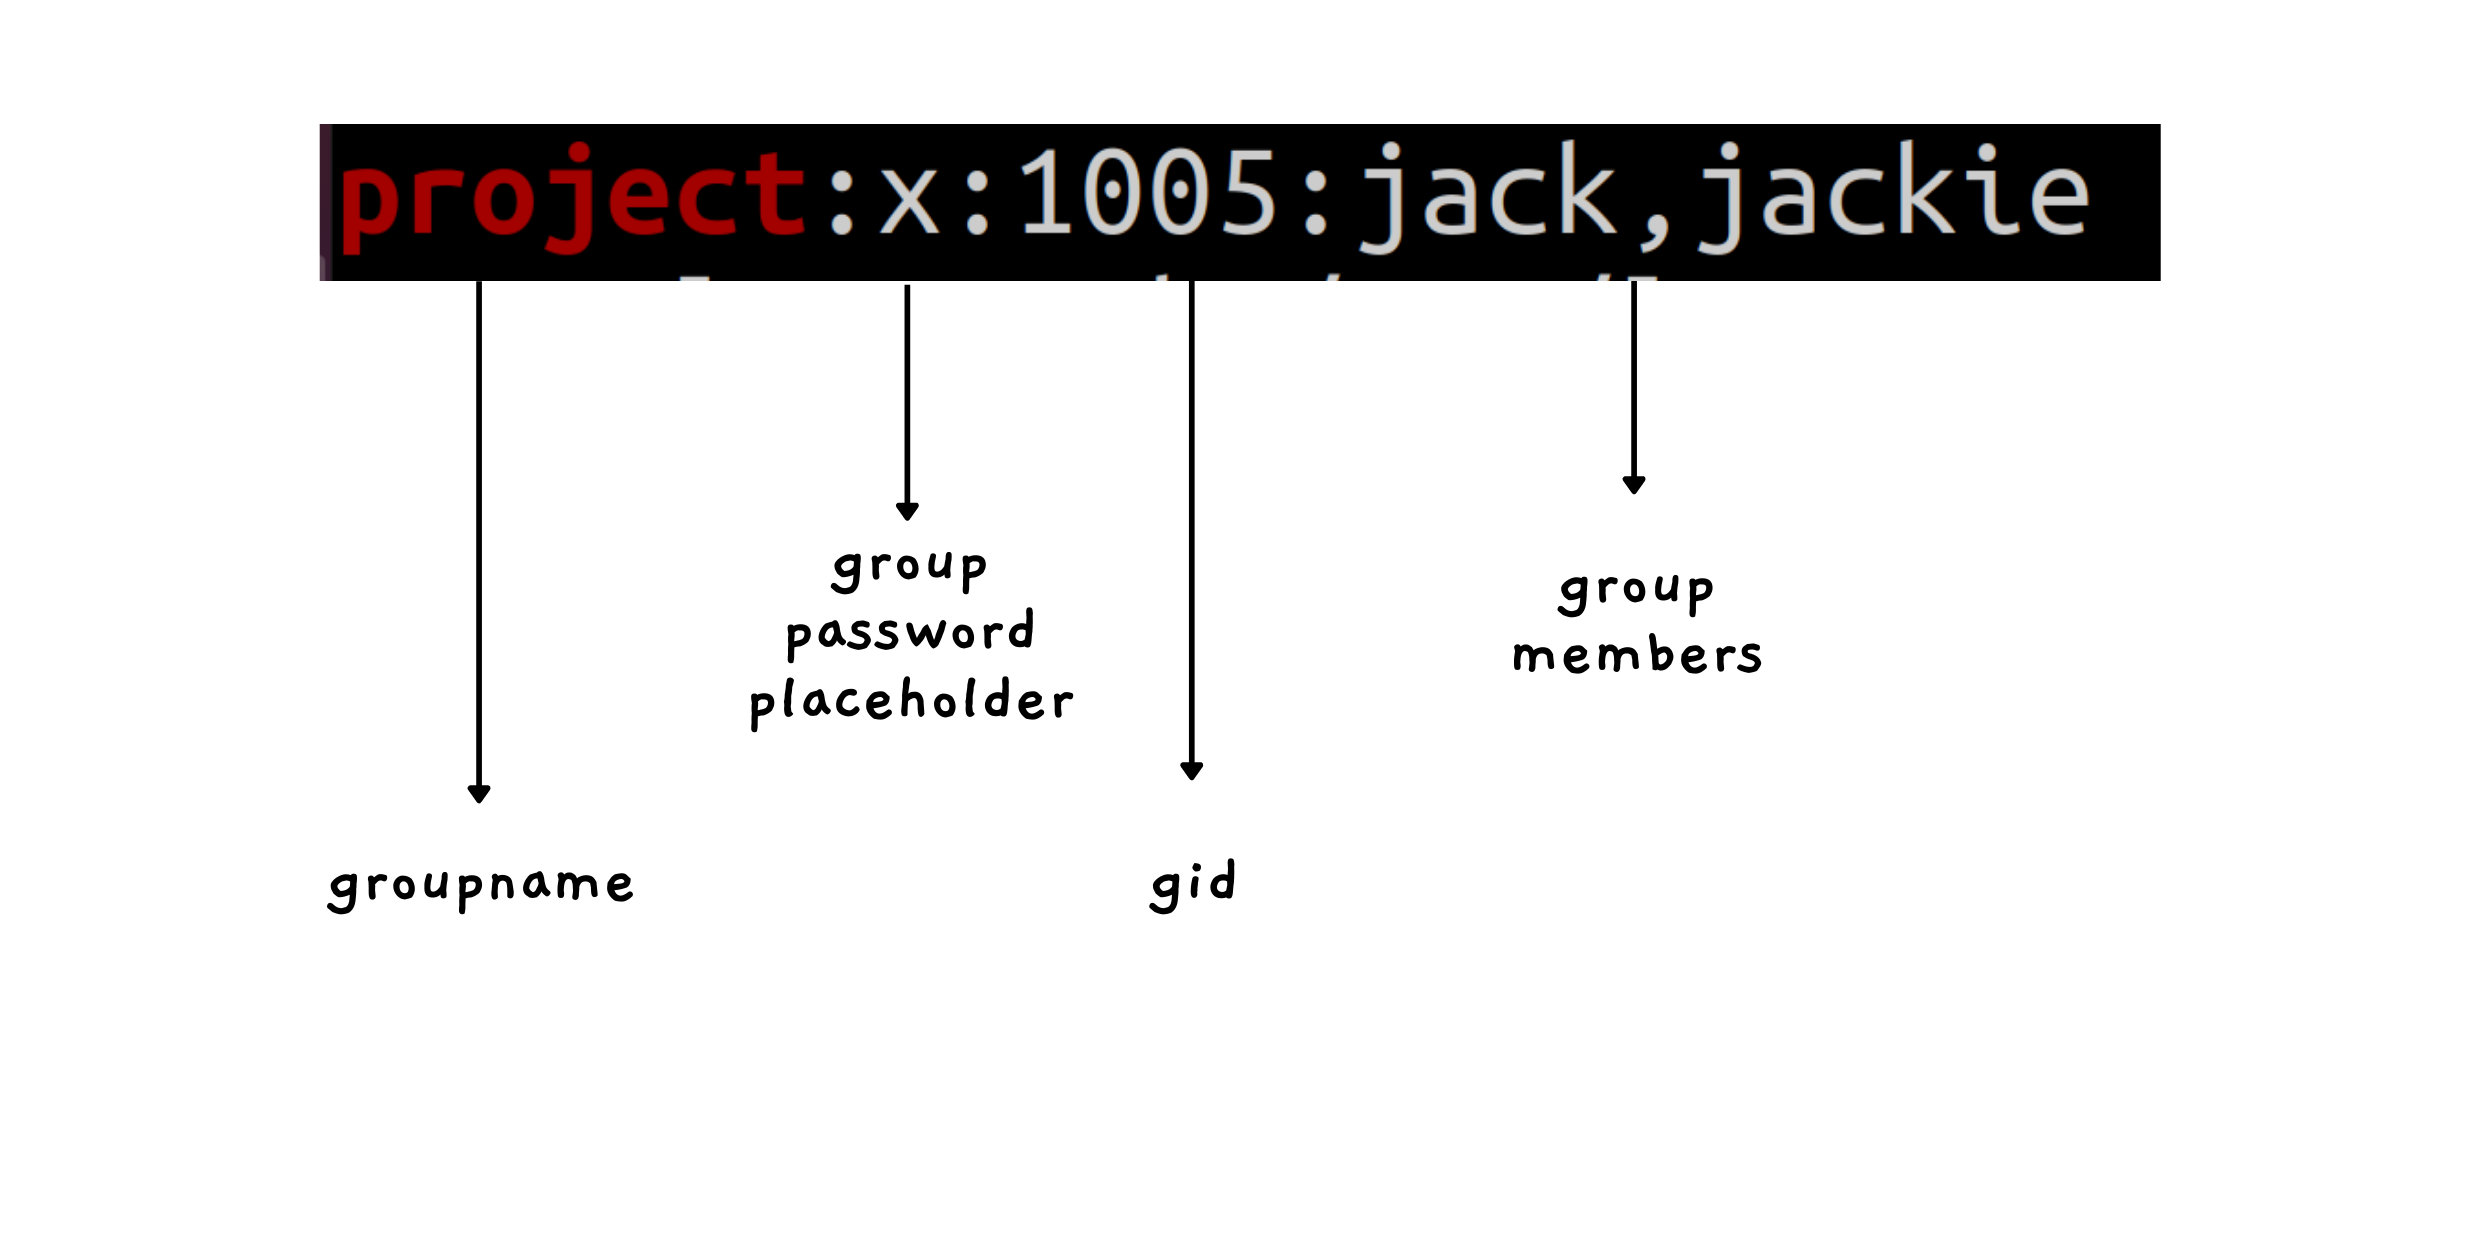
\includegraphics[scale=.2]{content/chapter4/images/54.png}
		\caption{Sample /etc/group entry}
		\label{fig:user_group}
	\end{figure}	
	\newline
	Explaination
	\begin{itemize}
		\item Column 1: \textbf{Groupname} - Name of group. It is case-sensitive. 
		\item Column 2: \textbf{Group password placeholder} - "x" acts as placeholder. Encrypted password are stored in \textbf{/etc/gshadow} file.
		\item Column 3: \textbf{Group ID} 
		\item Column 4: \textbf{Group members} - Usernames of users belonging to this group.
	\end{itemize}	
\end{itemize}	

\newpage
\textbf{Structure of the /etc/gshadow file}
\begin{itemize}
	\item Fields in this file are separated by a ":" (colon).
	\begin{figure}[h!]
		\centering
		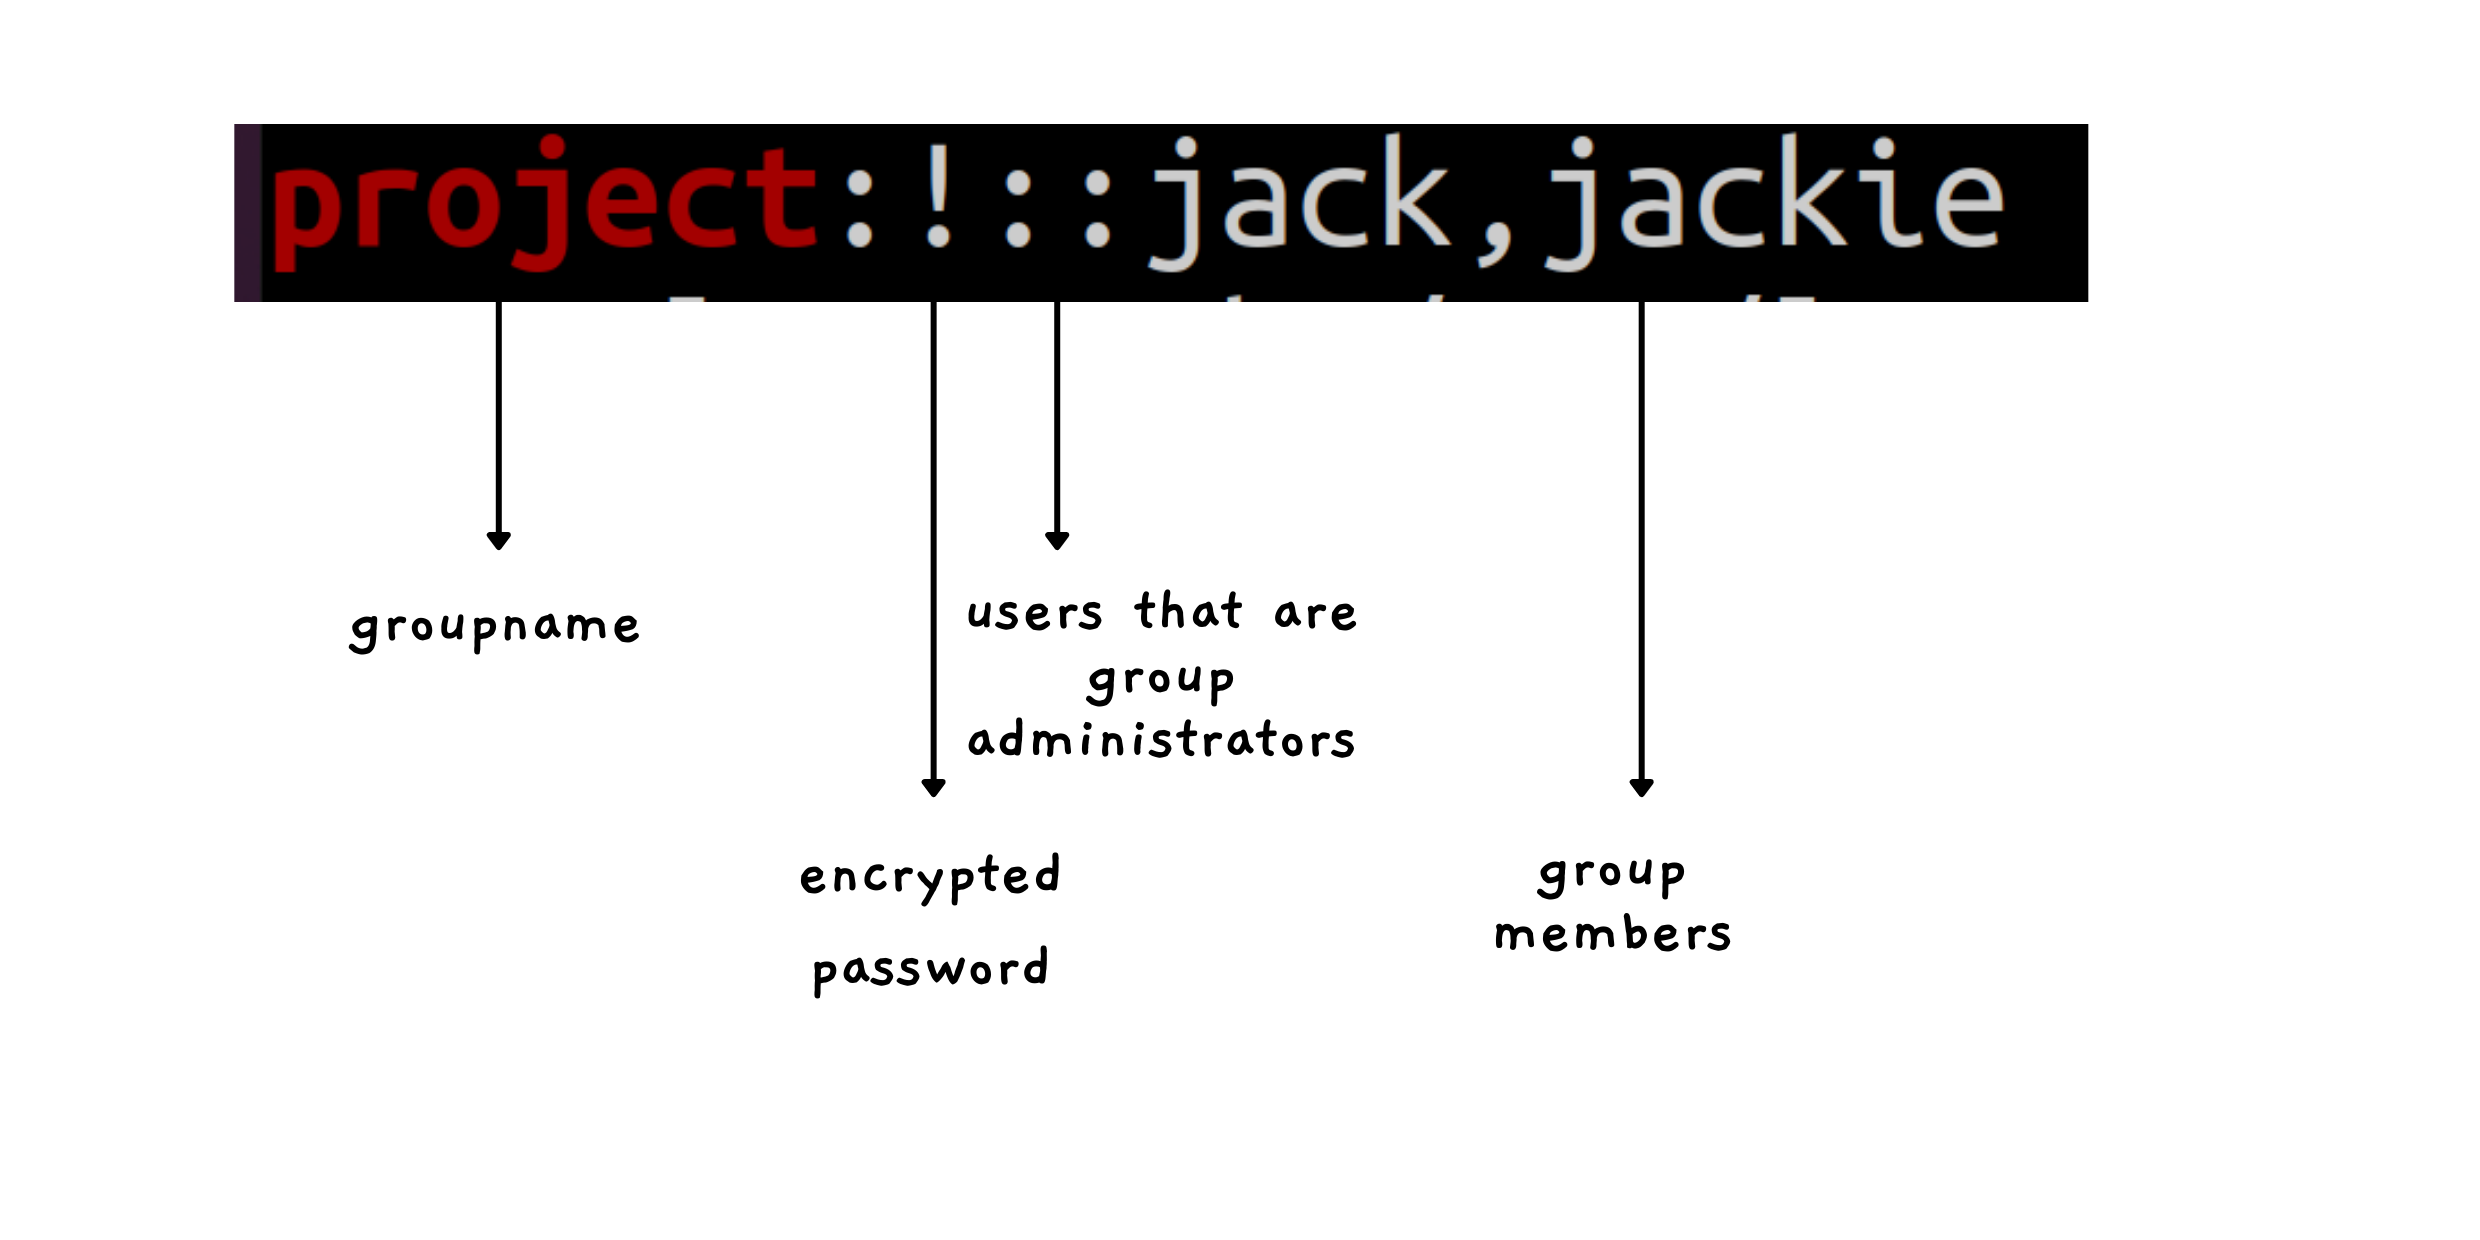
\includegraphics[scale=.2]{content/chapter4/images/56.png}
		\caption{Sample /etc/gshadow entry}
		\label{fig:user_group}
	\end{figure}	
	\newline
	Explaination:
	\begin{itemize}
		\item Column 1: \textbf{Groupname} - Name of group. It is case-sensitive. 
		\item Column 2: \textbf{Encrypted Password} - Store password in encrypted format.
		\bigskip
		\begin{tcolorbox}[breakable,notitle,boxrule=-0pt,colback=yellow,colframe=yellow]
			\color{black}
			\textbf{Note:} 
			\begin{itemize}
				\item {“!”} in this entry means the account is disabled or locked. 
				\item {“!!”} mask means password is not assigned.
			\end{itemize}
		\end{tcolorbox}

		\item Column 3: \textbf{Administrators} - Users who can change the password.
		\item Column 4: \textbf{Group members} - Usernames of user belonging to this group.
	\end{itemize}	
\end{itemize}	

	
\end{flushleft}

\newpage

